\chapter{Mutations and Genome Diversification}\label{ch:b2:genome-diversification}

Spread a billion bacteria on a plate laced with an antibiotic and,
the next morning, a handful of colonies have grown. Did the drug
teach those cells to resist it, or were they already resistant
before they met it? The question sounds philosophical and was
settled by an experiment of great elegance in 1943: the resistant
cells were there beforehand, produced by \omterm{def:b2:genome-diversification:mutation}{mutations} that happened at
random, without regard to their usefulness. This chapter is about the
sources of that variation --- the copying errors, the chemical
accidents, the jumping genes, the genes traded between cells, the
duplications of genes and of whole genomes --- and about how fast
they run. Selection, which sorts the variation, is the subject of
\cref{ch:b2:population-genetics}; here the subject is where the raw
material comes from.

\section{Mutations}

\begin{definition}[Mutation, and its kinds]\label{def:b2:genome-diversification:mutation}
\index{mutation}\index{point mutation}\index{frameshift}\index{chromosomal rearrangement}
A \emph{mutation} is a heritable change in the sequence of the
genome. \emph{Point mutations} change one or a few bases: a
\emph{substitution} replaces one base by another (a
\emph{transition} swaps purine for purine or pyrimidine for
pyrimidine, A$\leftrightarrow$G or C$\leftrightarrow$T; a
\emph{transversion} swaps the classes); an \emph{insertion} or
\emph{deletion} adds or removes bases. In a coding sequence a
substitution is \emph{silent} if the new codon specifies the same
amino acid, \emph{missense} if it specifies another, \emph{nonsense}
if it creates a stop; an insertion or deletion not a multiple of
three shifts the reading frame (\emph{frameshift}) and garbles every
codon downstream. \emph{Chromosomal rearrangements} move large
segments: deletion, duplication, inversion, translocation between
chromosomes. \emph{Genome mutations} change the number of
chromosomes: \emph{aneuploidy} (one chromosome too many or too few,
as in trisomy 21) and \emph{\omterm{def:b2:genome-diversification:polyploidy}{polyploidy}} (whole extra sets). A
mutation in a somatic cell is inherited by that cell's descendants
only; a mutation in the germ line is inherited by the organism's
descendants, and only these matter for evolution.
\end{definition}

\begin{omfigure}
\begin{tikzpicture}[every node/.style={font=\small\ttfamily}]
  \node[anchor=west] at (0,2.4) {ATG GAA TTC CTG AAG TGG TAA};
  \node[anchor=west, font=\scriptsize\rmfamily] at (5.6,2.4) {Met Glu Phe Leu Lys Trp stop --- wild type};
  \node[anchor=west] at (0,1.7) {ATG GA\textcolor{omThm}{G} TTC CTG AAG TGG TAA};
  \node[anchor=west, font=\scriptsize\rmfamily] at (5.6,1.7) {Met Glu Phe Leu Lys Trp stop --- silent};
  \node[anchor=west] at (0,1.0) {ATG G\textcolor{omThm}{T}A TTC CTG AAG TGG TAA};
  \node[anchor=west, font=\scriptsize\rmfamily] at (5.6,1.0) {Met \textcolor{omThm}{Val} Phe Leu Lys Trp stop --- missense};
  \node[anchor=west] at (0,0.3) {ATG \textcolor{omThm}{T}AA TTC CTG AAG TGG TAA};
  \node[anchor=west, font=\scriptsize\rmfamily] at (5.6,0.3) {Met \textcolor{omThm}{stop} --- nonsense};
  \node[anchor=west] at (0,-0.4) {ATG GA\textcolor{omThm}{C}A TTC CTG AAG TGG TAA};
  \node[anchor=west, font=\scriptsize\rmfamily] at (5.6,-0.4) {Met \textcolor{omThm}{Asp Ile Pro Glu Val} \dots{} --- frameshift};
\end{tikzpicture}

{\small \omterm{def:b2:genome-diversification:mutation}{Point mutations} in a short coding sequence (change in red).
A silent substitution keeps the protein; a missense changes one
residue; a nonsense truncates it; a single inserted base shifts the
frame and rewrites everything downstream.}
\end{omfigure}

\begin{proposition}[Where mutations come from]\label{prop:b2:genome-diversification:sources}
\index{mutagen}\index{deamination}\index{depurination}
Three sources. \emph{Replication errors}: DNA polymerase misplaces a
base about once in $10^{5}$; its proofreading exonuclease removes
most, leaving one in $10^{7}$; mismatch repair, which follows the
replication fork and corrects the new strand against the old, brings
the final error rate to about $10^{-9}$ to $10^{-10}$ per base per
replication. \emph{Spontaneous chemistry}: every day, in each human
cell, some \num{10000} purines fall off their sugars
(\emph{depurination}) and a hundred cytosines lose an amino group
(\emph{deamination}, turning C into U, which pairs with A); both are
repaired, but not always. \emph{Mutagens}: ultraviolet light welds
adjacent thymines into dimers; ionising radiation breaks strands;
alkylating agents and nitrous acid alter bases; intercalating dyes
slip between base pairs and cause \omterm{def:b2:genome-diversification:mutation}{frameshifts}; oxygen radicals from
respiration oxidise guanine. The rate per base is tiny; multiplied
by the size of a genome and the number of cells, it is not.
\end{proposition}

\begin{theorem}[Mutations per genome and per population]\label{thm:b2:genome-diversification:rate}
\index{mutation rate}
If the \omterm{thm:b2:genome-diversification:rate}{mutation rate} is $u$ per base pair per replication and the
genome holds $G$ base pairs, each replication produces on average
$U = uG$ new \omterm{def:b2:genome-diversification:mutation}{mutations}, and a population of $N$ cells produces $UN$
per generation. For \emph{E.~coli} ($u \approx \qty{5e-10}{}$, $G =
\qty{4.6e6}{}$): $U \approx 0.002$, so one cell in five hundred
carries a new \omterm{def:b2:genome-diversification:mutation}{mutation} --- but a culture of $10^{9}$ cells makes two
million per generation, and every one of the $3G \approx 1.4\times
10^{7}$ possible single-base changes arises somewhere in it every
few generations. For a human ($u \approx \qty{1.2e-8}{}$ per
generation, $G = \qty{3.2e9}{}$ per haploid set, two sets): each
child carries about \num{75} new \omterm{def:b2:genome-diversification:mutation}{mutations}, one or two of them in
coding sequence.
\end{theorem}
\begin{proof}
Each base is copied independently with probability $u$ of error, so
the number of errors per genome copy is a sum of $G$ independent
rare events, of mean $uG$ (and approximately Poisson distributed).
$N$ cells make $N$ copies. The human figure multiplies $u$ by $2G$
for the diploid genome; the rate per generation is per generation,
not per replication, because germ cells undergo many replications
between fertilisation and the next.
\end{proof}

\begin{theorem}[Mutants in a growing culture]\label{thm:b2:genome-diversification:luria}
\index{Luria--Delbr\"uck experiment}\index{fluctuation test}
A culture grown from $N_0$ to $N$ cells, in which a given \omterm{def:b2:genome-diversification:mutation}{mutation}
occurs with probability $m$ at each cell division, contains at the
end a mean number of \omterm{def:b2:genome-diversification:mutation}{mutation} \emph{events} $m(N - N_0)$, and a mean
number of mutant \emph{cells}
\[
\langle M\rangle = m\,N\,\ln\frac{N}{N_0},
\]
larger than the number of events because an early \omterm{def:b2:genome-diversification:mutation}{mutation} founds a
clone. The number of mutant cells varies enormously from culture to
culture (rare early events give ``jackpots''), whereas if the
\omterm{def:b2:genome-diversification:mutation}{mutations} were induced at plating, it would follow a Poisson law
with variance equal to its mean. The fraction of cultures with no
mutant at all is $p_0 = e^{-m(N - N_0)}$, which gives $m$ directly.
\end{theorem}
\begin{proof}
Growth from $n$ to $n + \mathrm{d}n$ cells takes $\mathrm{d}n$
divisions, each an opportunity for the \omterm{def:b2:genome-diversification:mutation}{mutation}, so $m\,\mathrm{d}n$
events occur in that interval; summing, $m(N - N_0)$ events in all.
A \omterm{def:b2:genome-diversification:mutation}{mutation} occurring when the culture has $n$ cells founds a clone
that grows in step with the culture and numbers $N/n$ cells at the
end; the expected number of mutant cells is therefore
$\int_{N_0}^{N} m\,(N/n)\,\mathrm{d}n = mN\ln(N/N_0)$. The events
are rare and independent, so their number is Poisson with mean
$m(N - N_0)$, and the probability of none is $e^{-m(N - N_0)}$.
\end{proof}
\begin{proof}[Evidence]
Luria and Delbr\"uck (1943) grew twenty small cultures of
\emph{E.~coli} from a few cells each, and in parallel took twenty
samples from one large culture; they plated all forty with a
bacteriophage that kills every sensitive cell and counted the
resistant colonies. The samples from the single culture gave counts
close to their mean, as a Poisson law predicts; the independent
cultures gave counts of 0, 0, 1, 0, 3, 0, 107, 0, 5\dots{} --- a
variance many times the mean. \omterm{def:b2:genome-diversification:mutation}{Mutations} to resistance had happened
at random times \emph{before} the cells met the phage, early ones
producing jackpots. Lederberg and Lederberg (1952) confirmed it
without ever exposing the selected cells to the agent: pressing a
velvet pad on a plate and stamping copies, they found resistant
colonies at the same positions on every replica, and isolated them
from the untreated master plate.
\end{proof}

\begin{omfigure}
\begin{tikzpicture}[every node/.style={font=\scriptsize}, level distance=0.55cm, sibling distance=0.5cm, edge from parent/.style={draw, gray}]
  \begin{scope}
    \node[circle, fill=omDef!40, inner sep=1.5pt] (r) at (0,0) {}
      child { node[circle, fill=omDef!40, inner sep=1.5pt] {}
        child { node[circle, fill=omDef!40, inner sep=1.5pt] {} child { node[circle, fill=omDef!40, inner sep=1.5pt] {} } child { node[circle, fill=omDef!40, inner sep=1.5pt] {} } }
        child { node[circle, fill=omDef!40, inner sep=1.5pt] {} child { node[circle, fill=omDef!40, inner sep=1.5pt] {} } child { node[circle, fill=omThm, inner sep=1.5pt] {} } } }
      child { node[circle, fill=omDef!40, inner sep=1.5pt] {}
        child { node[circle, fill=omDef!40, inner sep=1.5pt] {} child { node[circle, fill=omDef!40, inner sep=1.5pt] {} } child { node[circle, fill=omDef!40, inner sep=1.5pt] {} } }
        child { node[circle, fill=omDef!40, inner sep=1.5pt] {} child { node[circle, fill=omDef!40, inner sep=1.5pt] {} } child { node[circle, fill=omDef!40, inner sep=1.5pt] {} } } };
    \node[align=center] at (0,-2.4) {late mutation:\\one mutant cell};
  \end{scope}
  \begin{scope}[xshift=5cm]
    \node[circle, fill=omDef!40, inner sep=1.5pt] at (0,0) {}
      child { node[circle, fill=omThm, inner sep=1.5pt] {}
        child { node[circle, fill=omThm, inner sep=1.5pt] {} child { node[circle, fill=omThm, inner sep=1.5pt] {} } child { node[circle, fill=omThm, inner sep=1.5pt] {} } }
        child { node[circle, fill=omThm, inner sep=1.5pt] {} child { node[circle, fill=omThm, inner sep=1.5pt] {} } child { node[circle, fill=omThm, inner sep=1.5pt] {} } } }
      child { node[circle, fill=omDef!40, inner sep=1.5pt] {}
        child { node[circle, fill=omDef!40, inner sep=1.5pt] {} child { node[circle, fill=omDef!40, inner sep=1.5pt] {} } child { node[circle, fill=omDef!40, inner sep=1.5pt] {} } }
        child { node[circle, fill=omDef!40, inner sep=1.5pt] {} child { node[circle, fill=omDef!40, inner sep=1.5pt] {} } child { node[circle, fill=omDef!40, inner sep=1.5pt] {} } } };
    \node[align=center] at (0,-2.4) {early mutation:\\a jackpot of four};
  \end{scope}
  \begin{scope}[xshift=10cm]
    \node[circle, fill=omDef!40, inner sep=1.5pt] at (0,0) {}
      child { node[circle, fill=omDef!40, inner sep=1.5pt] {}
        child { node[circle, fill=omDef!40, inner sep=1.5pt] {} child { node[circle, fill=omDef!40, inner sep=1.5pt] {} } child { node[circle, fill=omThm, inner sep=1.5pt] {} } }
        child { node[circle, fill=omDef!40, inner sep=1.5pt] {} child { node[circle, fill=omDef!40, inner sep=1.5pt] {} } child { node[circle, fill=omDef!40, inner sep=1.5pt] {} } } }
      child { node[circle, fill=omDef!40, inner sep=1.5pt] {}
        child { node[circle, fill=omDef!40, inner sep=1.5pt] {} child { node[circle, fill=omThm, inner sep=1.5pt] {} } child { node[circle, fill=omDef!40, inner sep=1.5pt] {} } }
        child { node[circle, fill=omDef!40, inner sep=1.5pt] {} child { node[circle, fill=omDef!40, inner sep=1.5pt] {} } child { node[circle, fill=omDef!40, inner sep=1.5pt] {} } } };
    \node[align=center] at (0,-2.4) {if induced at plating:\\a Poisson scatter};
  \end{scope}
\end{tikzpicture}

{\small The \omterm{thm:b2:genome-diversification:luria}{fluctuation test}. If \omterm{def:b2:genome-diversification:mutation}{mutations} (red) occur at random
during growth, the number of mutants depends on \emph{when} the
\omterm{def:b2:genome-diversification:mutation}{mutation} happened, and independent cultures differ wildly; if the
selecting agent induced them at plating, every culture would show a
similar small number.}
\end{omfigure}

\begin{omfigure}
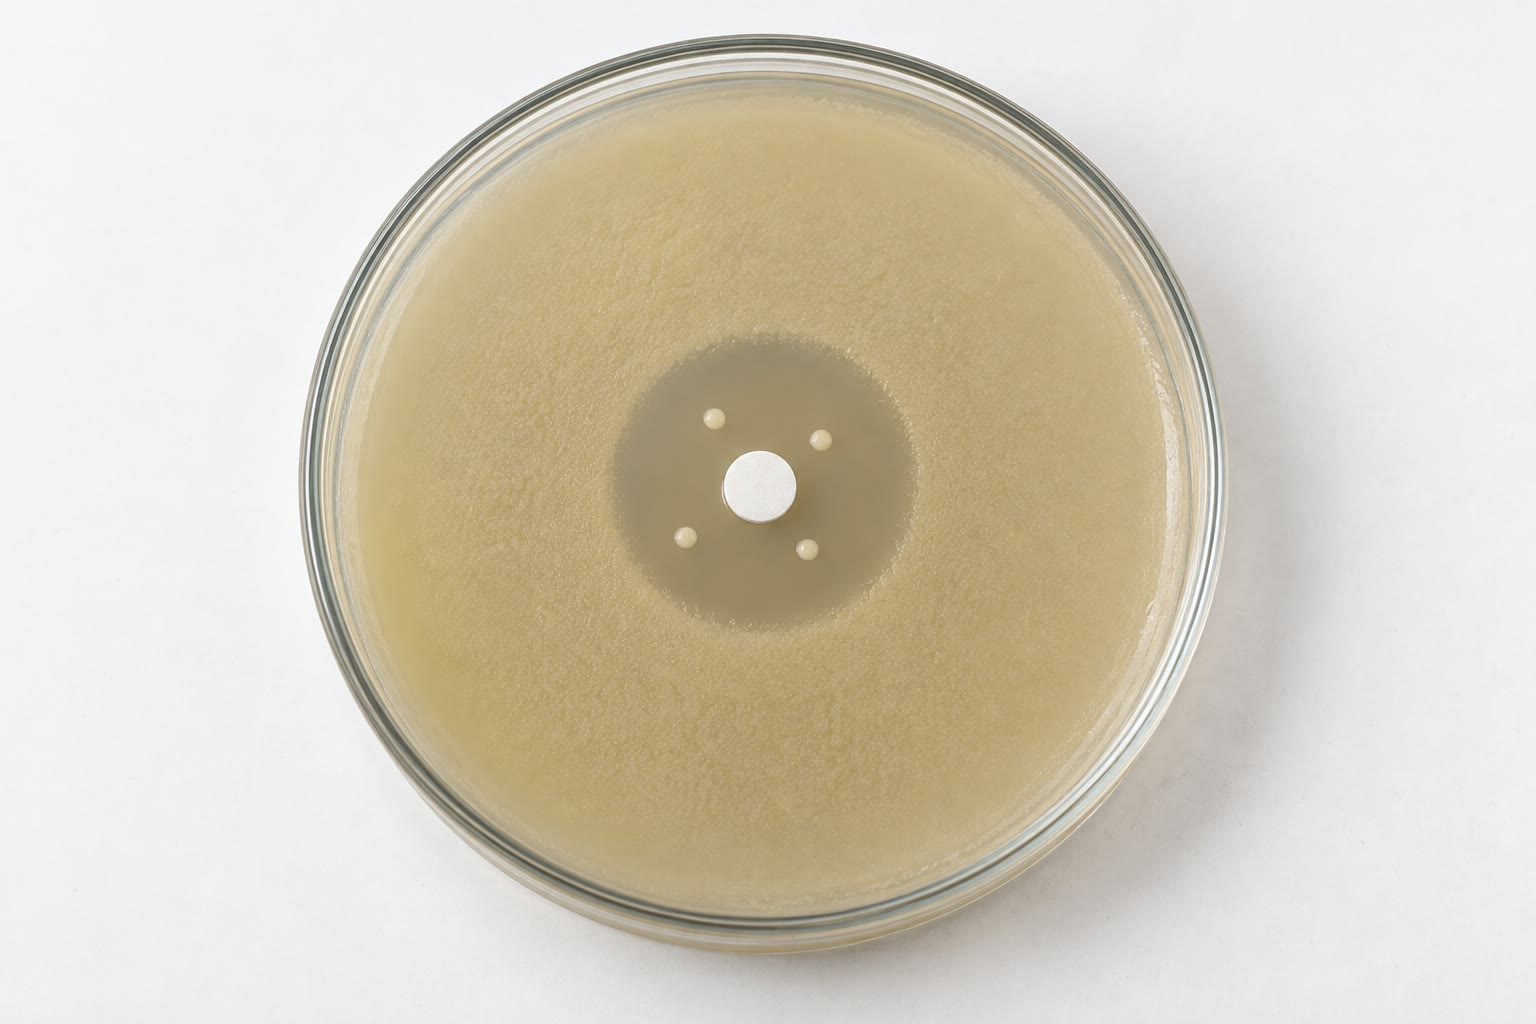
\includegraphics[width=0.5\linewidth]{images/book4/ai/b4-03-luria-plate.jpg}

{\small An antibiotic disc on a lawn of bacteria: the clear zone is
where the drug diffusing from the disc has killed the sensitive
cells, and the colonies inside it grew from resistant mutants that
were present before the disc was laid down.}
\end{omfigure}

\begin{proposition}[Repair, and its limits]\label{prop:b2:genome-diversification:repair}
\index{DNA repair}
A cell corrects most damage before it becomes a \omterm{def:b2:genome-diversification:mutation}{mutation}.
\emph{Mismatch repair} removes the wrong base from the newly made
strand. \emph{Base excision repair} cuts out a single damaged base
(a uracil, an oxidised guanine) and fills the gap; it is why DNA
uses thymine rather than uracil: a uracil in DNA can only be a
deaminated cytosine, and is recognised as foreign. \emph{Nucleotide
excision repair} removes a stretch of a dozen bases around a bulky
lesion such as a thymine dimer; people lacking it (xeroderma
pigmentosum) develop skin cancers from ordinary sunlight.
\emph{Recombinational repair} rebuilds a broken chromosome from its
sister copy. What escapes repair, or is repaired wrongly, is a
\omterm{def:b2:genome-diversification:mutation}{mutation} --- and a cell that has lost a repair system (a
\emph{mutator}) mutates a hundred times faster, which is a
short-term advantage under stress and a long-term burden. Repair
mechanisms are treated in depth in the Year 3 volume.
\end{proposition}

\section{Genes that move}

\begin{definition}[Transposable elements]\label{def:b2:genome-diversification:transposon}
\index{transposon}\index{retrotransposon}
A \emph{transposable element} is a DNA segment that can move to a
new position in the genome. \emph{DNA transposons} encode a
\emph{transposase} that cuts the element out and pastes it elsewhere
(or copies it there); bacterial insertion sequences are the simplest
(a transposase gene between two inverted repeats), and composite
transposons carry extra genes --- often antibiotic resistances ---
between two of them. \emph{Retrotransposons} move by a copy-and-paste
route through an RNA intermediate, copied back into DNA by a reverse
transcriptase; they never leave their old site and so accumulate.
An element landing in a gene disrupts it; landing near one, it may
alter its expression; two copies in one chromosome provide sites for
\omterm{prop:b2:genome-diversification:duplication}{unequal crossing-over}. Transposons and their relics make up half of
the human genome and eighty percent of the maize genome; most are
now immobile.
\end{definition}
\begin{proof}[Evidence]
McClintock (1940s--1950s) studied maize kernels whose purple
pigment was lost in some cells and restored in others, giving
speckled kernels. She showed by breeding and by chromosome
observation that the instability was caused by an element
(\emph{Dissociation}) that broke the chromosome where it sat and
moved between positions under the control of a second element
(\emph{Activator}), and that a gene was silenced when the element
sat in it and reactivated when it left. Genes, she concluded, could
change position; the idea was accepted only twenty years later, when
bacterial insertion sequences were found, and earned her a Nobel
Prize in 1983.
\end{proof}

\begin{omfigure}
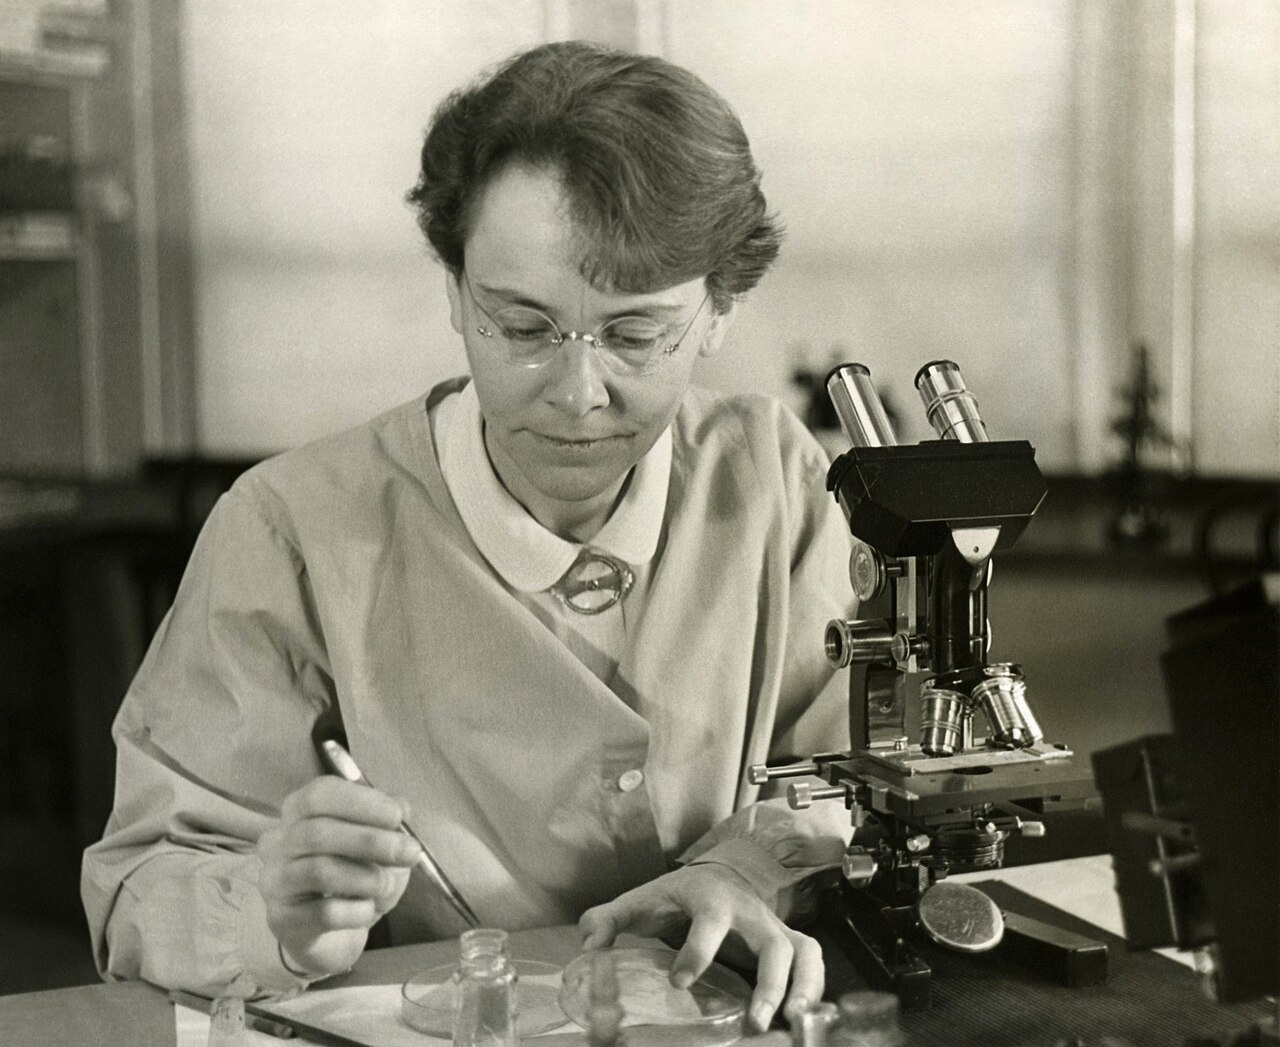
\includegraphics[width=0.4\linewidth]{images/book4/mcclintock.jpg}\hspace{0.04\linewidth}
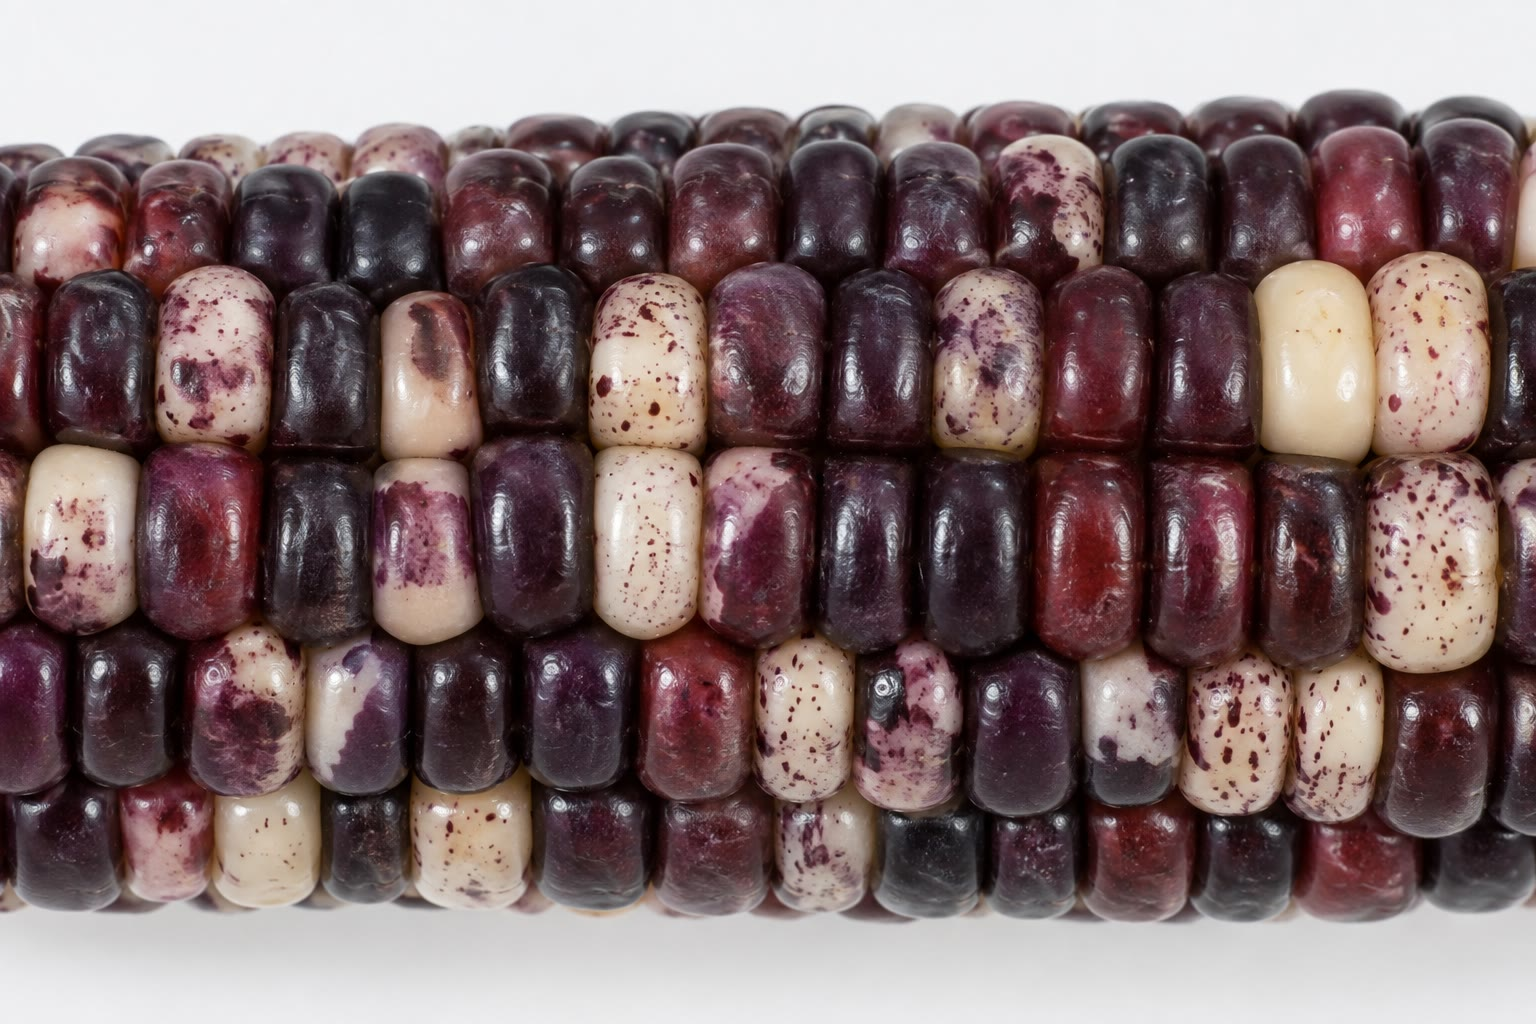
\includegraphics[width=0.5\linewidth]{images/book4/ai/b4-03-maize-kernels.jpg}

{\small Barbara McClintock, and the kernels that led her to
transposable elements: a purple pigment gene switched off by an
inserted element and switched back on, cell by cell, when the
element jumps out, leaving speckles and sectors.}
\end{omfigure}

\begin{omfigure}
\begin{tikzpicture}[every node/.style={font=\scriptsize}]
  % cut and paste
  \begin{scope}
    \draw[very thick, gray] (0,1.2) -- (4.5,1.2);
    \fill[omThm!70] (0.8,1.05) rectangle (1.8,1.35); \node[white, font=\tiny] at (1.3,1.2) {Tn};
    \draw[very thick, gray] (0,0) -- (4.5,0);
    \fill[omThm!70] (2.8,-0.15) rectangle (3.8,0.15); \node[white, font=\tiny] at (3.3,0) {Tn};
    \draw[->, thick, omThm] (1.3,1.0) .. controls (1.3,0.5) and (3.3,0.7) .. (3.3,0.2);
    \draw[dashed, gray] (0.8,1.2) -- (1.8,1.2);
    \node[align=center] at (2.25,-0.6) {cut and paste (DNA transposon):\\the element leaves its old site};
  \end{scope}
  % copy and paste
  \begin{scope}[xshift=7.5cm]
    \draw[very thick, gray] (0,1.2) -- (4.5,1.2);
    \fill[omProp!80] (0.8,1.05) rectangle (1.8,1.35); \node[white, font=\tiny] at (1.3,1.2) {RT};
    \draw[very thick, gray] (0,0) -- (4.5,0);
    \fill[omProp!80] (2.8,-0.15) rectangle (3.8,0.15); \node[white, font=\tiny] at (3.3,0) {RT};
    \draw[->, thick, omProp] (1.3,1.0) .. controls (1.3,0.5) and (3.3,0.7) .. (3.3,0.2);
    \node[omProp, anchor=west, align=left] at (3.6,0.75) {RNA copy,\\reverse transcribed};
    \node[align=center] at (2.25,-0.6) {copy and paste (retrotransposon):\\the old copy stays, the number grows};
  \end{scope}
\end{tikzpicture}

{\small Two ways to move. A DNA \omterm{def:b2:genome-diversification:transposon}{transposon} is excised and
reinserted; a \omterm{def:b2:genome-diversification:transposon}{retrotransposon} is transcribed, copied back into DNA
and inserted elsewhere, so that its copies accumulate.}
\end{omfigure}

\begin{definition}[Horizontal gene transfer]\label{def:b2:genome-diversification:hgt}
\index{horizontal gene transfer}\index{transformation}\index{conjugation!bacterial}\index{transduction}
\omterm{def:b2:unicellular-diversity:prokaryote}{Prokaryotes} acquire genes from cells that are not their parents by
three routes. \emph{Transformation}: a cell takes up naked DNA from
its surroundings (released by dead cells) and recombines it into its
chromosome; some species are naturally competent, and it is the
route by which pneumococci exchange capsule genes. \emph{Conjugation}:
a donor carrying a conjugative \omterm{def:b2:unicellular-diversity:prokaryote}{plasmid} (the F factor of
\emph{E.~coli}) builds a pilus, draws a recipient close, and passes a
single strand of the \omterm{def:b2:unicellular-diversity:prokaryote}{plasmid} through a pore while replicating it by
the rolling circle; if the \omterm{def:b2:unicellular-diversity:prokaryote}{plasmid} has integrated into the
chromosome (an Hfr strain), chromosomal genes are transferred in
order behind it, and the time at which each enters maps the
chromosome. \emph{Transduction}: a bacteriophage packages a piece of
host DNA by mistake and injects it into the next cell it infects.
Together these routes move resistance genes between species within
hospitals in years, and have moved metabolic genes across the whole
bacterial tree over geological time, so that a \omterm{def:b2:unicellular-diversity:prokaryote}{prokaryote}'s
ancestry is a web as much as a tree
(\cref{ch:b2:phylogenetic-trees}).
\end{definition}
\begin{proof}[Evidence]
Lederberg and Tatum (1946) mixed two strains of \emph{E.~coli}, each
unable to make two different nutrients, and plated the mixture on a
minimal medium on which neither could grow alone: colonies appeared,
at about one per ten million cells, that could make all four ---
recombinants. Davis (1950) repeated it with the strains separated by
a filter that let molecules through but not cells: no recombinants,
so contact was needed. Hayes then showed the transfer was one-way,
from a donor to a recipient, and Wollman and Jacob (1956)
interrupted matings in a blender at intervals and found the donor's
genes entering the recipient in a fixed order, one after another,
over about a hundred minutes.
\end{proof}

\begin{omfigure}
\begin{minipage}[b]{0.56\linewidth}\centering
\begin{tikzpicture}[every node/.style={font=\scriptsize}]
  % donor
  \draw[thick, fill=omDef!8] (0,0) ellipse (1.5 and 0.75);
  \draw[thick, omDef] (0.2,0) circle (0.45);
  \draw[thick, omThm] (-0.9,0.1) circle (0.22);
  \node[anchor=south] at (0,1.25) {donor $F^+$};
  \draw[omThm] (-0.9,-0.12) -- (-1.1,-1.0) node[below] {F plasmid};
  \draw[omDef] (0.4,-0.4) -- (0.6,-1.0) node[below] {chromosome};
  % recipient
  \draw[thick, fill=omDef!8] (5,0) ellipse (1.5 and 0.75);
  \draw[thick, omDef] (5.2,0) circle (0.45);
  \node[anchor=south] at (5,1.25) {recipient $F^-$};
  % pilus
  \draw[very thick, omThm] (1.5,0) -- (3.5,0);
  \node[omThm, below] at (2.5,-0.05) {pilus};
  % single strand transferred
  \draw[->, thick, omThm, dashed] (-0.7,0.15) .. controls (1.0,0.7) and (3.0,0.7) .. (4.1,0.4);
  \node[omThm, anchor=south] at (2.5,0.7) {one strand copied by rolling circle};
  \draw[thick, omThm, dashed] (4.1,0.2) circle (0.2);
\end{tikzpicture}
\end{minipage}\hfill
\begin{minipage}[b]{0.42\linewidth}\centering
\begin{tikzpicture}
\begin{axis}[
  width=\linewidth, height=4.6cm,
  axis x line=bottom, axis y line=left,
  xmin=0, xmax=40, ymin=0, ymax=1.1,
  xlabel={minutes before blending}, ylabel={recombinants (relative)},
  xlabel style={font=\scriptsize, at={(axis description cs:0.5,-0.18)}, anchor=north},
  ylabel style={font=\scriptsize},
  tick label style={font=\scriptsize}, xtick={0,10,20,30,40}, ytick={0,0.5,1},
  legend style={font=\scriptsize, at={(0.97,0.08)}, anchor=south east, draw=none},
  clip=false,
]
\addplot[very thick, omDef, domain=8:40, samples=40] {1-exp(-(x-8)/5)};
\addlegendentry{\emph{thr}, enters at \qty{8}{min}}
\addplot[very thick, omProp, domain=17:40, samples=40] {1-exp(-(x-17)/5)};
\addlegendentry{\emph{lac}, \qty{17}{min}}
\addplot[very thick, omThm, domain=25:40, samples=40] {1-exp(-(x-25)/5)};
\addlegendentry{\emph{gal}, \qty{25}{min}}
\end{axis}
\end{tikzpicture}
\end{minipage}

{\small Left: conjugation --- the donor passes one strand of its F
\omterm{def:b2:unicellular-diversity:prokaryote}{plasmid} through the pilus junction while copying it. Right: the
interrupted-mating experiment with an Hfr donor: each chromosomal
gene begins to appear among recombinants at a characteristic time,
which maps the chromosome in minutes.}
\end{omfigure}

\begin{omfigure}
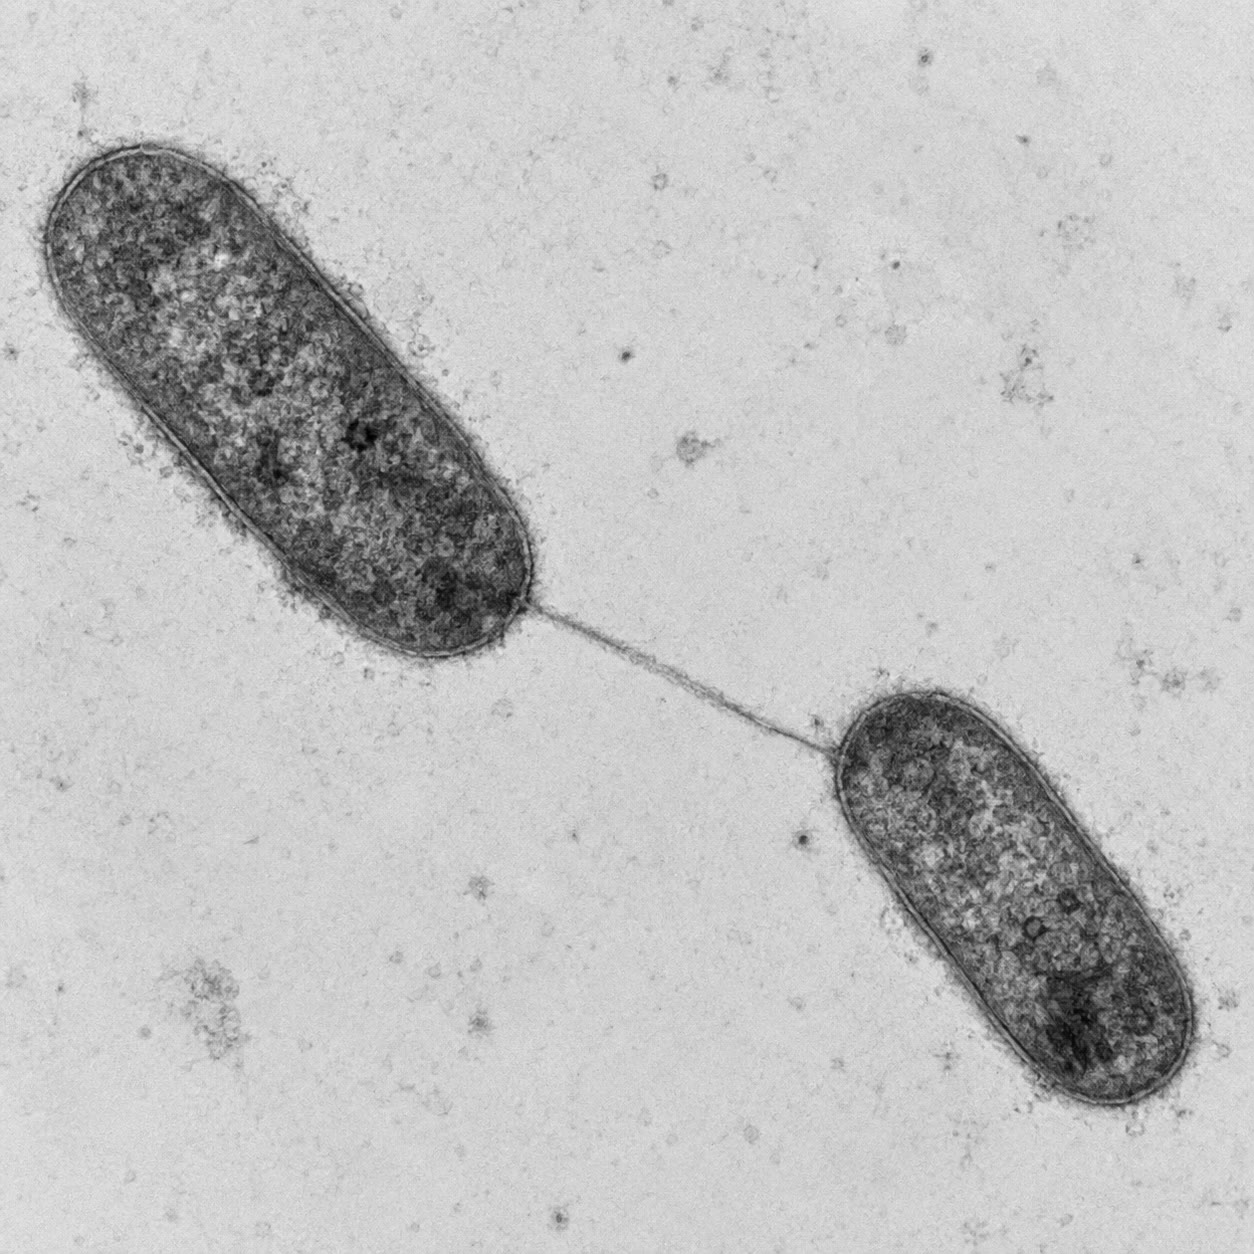
\includegraphics[width=0.42\linewidth]{images/book4/ai/b4-03-conjugation-tem.jpg}

{\small Two bacteria joined by a conjugative pilus, seen by
transmission electron microscopy: the bridge along which the \omterm{def:b2:unicellular-diversity:prokaryote}{plasmid}
passes.}
\end{omfigure}

\begin{example}[Resistance on the move]\label{ex:b2:genome-diversification:resistance}
A resistance gene typically arises once, by \omterm{def:b2:genome-diversification:mutation}{mutation} or from the
soil bacterium that makes the antibiotic, and then travels: from a
chromosome onto a \omterm{def:b2:genome-diversification:transposon}{transposon}, from the \omterm{def:b2:genome-diversification:transposon}{transposon} onto a
conjugative \omterm{def:b2:unicellular-diversity:prokaryote}{plasmid}, from the \omterm{def:b2:unicellular-diversity:prokaryote}{plasmid} across species by conjugation
and across strains by \omterm{def:b2:genome-diversification:hgt}{transduction}, and back into a chromosome by
\omterm{def:b2:genome-diversification:hgt}{transformation}. \omterm{def:b2:unicellular-diversity:prokaryote}{Plasmids} carrying five or six resistances at once
(assembled in \emph{integrons}, which capture gene cassettes) were
found in Japan in the 1950s, a few years after the drugs came into
use; the gene for the carbapenemase NDM-1, first seen in 2008,
reached every continent within three years on a \omterm{def:b2:unicellular-diversity:prokaryote}{plasmid}. The
evolution of resistance is mostly not the evolution of new genes but
the movement of old ones.
\end{example}

\section{Duplication: genes and genomes}

\begin{proposition}[Gene duplication and gene families]\label{prop:b2:genome-diversification:duplication}
\index{gene duplication}\index{gene family}\index{unequal crossing-over}
When two similar sequences sit in tandem on a chromosome, the
homologues may pair out of register at meiosis and cross over
unequally, so that one product carries three copies and the other
one. A duplicated gene is redundant: one copy can keep the old job
while the other accumulates \omterm{def:b2:genome-diversification:mutation}{mutations} freely --- usually decaying
into a \emph{pseudogene}, occasionally acquiring a new function
(\emph{neofunctionalisation}) or a share of the old one
(\emph{subfunctionalisation}). Repeated over hundreds of millions of
years this builds \emph{gene families}: the globins (a single
ancestral gene became myoglobin, the $\alpha$ cluster and the
$\beta$ cluster, with embryonic, fetal and adult members expressed
in turn), the olfactory receptors (a thousand genes in a mouse), the
homeobox genes, the crystallins of the lens. Most of the genes of a
genome belong to a family, and duplication is the main source of new
genes.
\end{proposition}
\begin{proof}[Evidence]
The human $\beta$-globin cluster on chromosome 11 holds five
functional genes ($\varepsilon$, $^{G}\gamma$, $^{A}\gamma$,
$\delta$, $\beta$) and a pseudogene, in the order in which they are
switched on during development, all with the same exon--intron
structure, their sequences more alike the more recently they
diverged; the $\alpha$ cluster on chromosome 16 has the same
architecture. Deletions of one or more $\alpha$ genes, produced by
\omterm{prop:b2:genome-diversification:duplication}{unequal crossing-over} between the near-identical copies, are common
and cause $\alpha$-thalassaemia; the reciprocal product, a
chromosome with three $\alpha$ genes, is found in the same
populations.
\end{proof}

\begin{omfigure}
\begin{tikzpicture}[every node/.style={font=\scriptsize}]
  % unequal crossing over
  \begin{scope}
    \draw[very thick, gray] (0,1.2) -- (5,1.2);
    \fill[omDef!70] (1.0,1.05) rectangle (2.0,1.35); \fill[omDef!70] (2.4,1.05) rectangle (3.4,1.35);
    \draw[very thick, gray] (0,0) -- (5,0);
    \fill[omDef!70] (1.0,-0.15) rectangle (2.0,0.15); \fill[omDef!70] (2.4,-0.15) rectangle (3.4,0.15);
    \node[above] at (1.5,1.35) {A}; \node[above] at (2.9,1.35) {A$'$};
    \draw[very thick, omThm] (2.9,1.05) -- (1.5,0.15);
    \node[align=center] at (2.5,-0.6) {mispaired homologues\\cross over unequally};
    \draw[->, thick, gray] (5.3,0.6) -- (6.1,0.6);
    % products
    \draw[very thick, gray] (6.5,1.2) -- (11.5,1.2);
    \fill[omDef!70] (7.5,1.05) rectangle (8.5,1.35); \fill[omDef!70] (8.9,1.05) rectangle (9.9,1.35); \fill[omDef!70] (10.3,1.05) rectangle (11.3,1.35);
    \node[above] at (9.4,1.35) {three copies};
    \draw[very thick, gray] (6.5,0) -- (11.5,0);
    \fill[omDef!70] (7.5,-0.15) rectangle (8.5,0.15);
    \node[above] at (8.0,0.15) {one copy};
  \end{scope}
  % globin family tree
  \begin{scope}[yshift=-3.6cm]
    \draw[thick] (2,2.2) -- (2,1.7);
    \draw[thick] (0.5,1.7) -- (3.5,1.7);
    \draw[thick] (0.5,1.7) -- (0.5,0.4); \node[below] at (0.5,0.4) {myoglobin};
    \draw[thick] (3.5,1.7) -- (3.5,1.2);
    \draw[thick] (2.3,1.2) -- (4.7,1.2);
    \draw[thick] (2.3,1.2) -- (2.3,0.4); \node[below] at (2.3,0.4) {$\alpha$ family};
    \draw[thick] (4.7,1.2) -- (4.7,0.9);
    \draw[thick] (3.6,0.9) -- (5.8,0.9);
    \draw[thick] (3.6,0.9) -- (3.6,0.4); \node[below] at (3.6,0.4) {$\varepsilon,\gamma$};
    \draw[thick] (5.8,0.9) -- (5.8,0.7);
    \draw[thick] (5.2,0.7) -- (6.4,0.7);
    \draw[thick] (5.2,0.7) -- (5.2,0.4); \node[below] at (5.2,0.4) {$\delta$};
    \draw[thick] (6.4,0.7) -- (6.4,0.4); \node[below] at (6.4,0.4) {$\beta$};
    \node[anchor=west, align=left] at (7.2,1.7) {duplications of one ancestral globin gene:\\before the vertebrates (myoglobin/haemoglobin),\\$\sim$450 million years ago ($\alpha$/$\beta$),\\then within the $\beta$ cluster (embryonic, fetal, adult)};
    \node[anchor=east, gray] at (1.9,2.1) {ancestral globin};
  \end{scope}
\end{tikzpicture}

{\small Above: \omterm{prop:b2:genome-diversification:duplication}{unequal crossing-over} between mispaired tandem copies
produces a chromosome with three copies and one with a single copy.
Below: the globin family, built by successive duplications and
divergence.}
\end{omfigure}

\begin{definition}[Polyploidy]\label{def:b2:genome-diversification:polyploidy}
\index{polyploidy}\index{allopolyploid}\index{autopolyploid}
A \emph{polyploid} carries more than two complete chromosome sets.
An \emph{autopolyploid} has several sets from one species (a failed
meiosis gives a diploid gamete; two such gametes give a
tetraploid); an \emph{allopolyploid} combines the sets of two species
after a hybridisation. The diploid hybrid AB, with no homologue for
any chromosome, cannot pair them at meiosis and is sterile; if its
genome doubles to AABB, every chromosome again has a partner, meiosis
works, and the new plant is fertile --- but cannot cross back with
either parent (an AAB offspring is sterile). Polyploidy thus makes a
new species in one step, and about a third of flowering-plant
species arose this way: bread wheat is a hexaploid AABBDD of three
grasses, the garden strawberry an octoploid, cotton and tobacco
allotetraploids, and the vertebrate lineage itself doubled its
genome twice near its origin. Polyploids are usually larger than
their diploid ancestors (more DNA, bigger cells) and much prized by
breeders.
\end{definition}

\begin{omfigure}
\begin{tikzpicture}[every node/.style={font=\scriptsize}]
  \node[draw, rounded corners, fill=omDef!10, align=center] (a) at (0,0) {\emph{T.~urartu}\\AA, $2n = 14$};
  \node[draw, rounded corners, fill=omDef!10, align=center] (b) at (3.4,0) {\emph{Aegilops}\\BB, $2n = 14$};
  \node[draw, rounded corners, fill=omProp!15, align=center] (ab) at (1.7,-1.5) {hybrid AB\\$n = 14$, sterile};
  \node[draw, rounded corners, fill=omExo!25, align=center] (aabb) at (1.7,-3.1) {emmer wheat AABB\\$2n = 28$, fertile};
  \node[draw, rounded corners, fill=omDef!10, align=center] (d) at (6.4,-3.1) {\emph{Ae.~tauschii}\\DD, $2n = 14$};
  \node[draw, rounded corners, fill=omProp!15, align=center] (abd) at (4.0,-4.6) {hybrid ABD\\$3n = 21$, sterile};
  \node[draw, rounded corners, fill=omExo!25, align=center] (abd2) at (4.0,-6.1) {bread wheat AABBDD\\$2n = 42$, fertile};
  \draw[->, thick] (a) -- (ab); \draw[->, thick] (b) -- (ab);
  \draw[->, thick] (ab) -- (aabb) node[midway, right] {genome doubling};
  \draw[->, thick] (aabb) -- (abd); \draw[->, thick] (d) -- (abd);
  \draw[->, thick] (abd) -- (abd2) node[midway, right] {genome doubling};
  \node[anchor=west, align=left, gray] at (7.8,-1.5) {each hybridisation gives a sterile\\plant with unpaired chromosomes;\\each doubling restores pairing\\and fertility --- and makes a\\species that cannot cross back};
\end{tikzpicture}

{\small The origin of bread wheat: two hybridisations, each followed
by a doubling of the genome, built a hexaploid from three diploid
grasses in about ten thousand years.}
\end{omfigure}

\begin{omfigure}
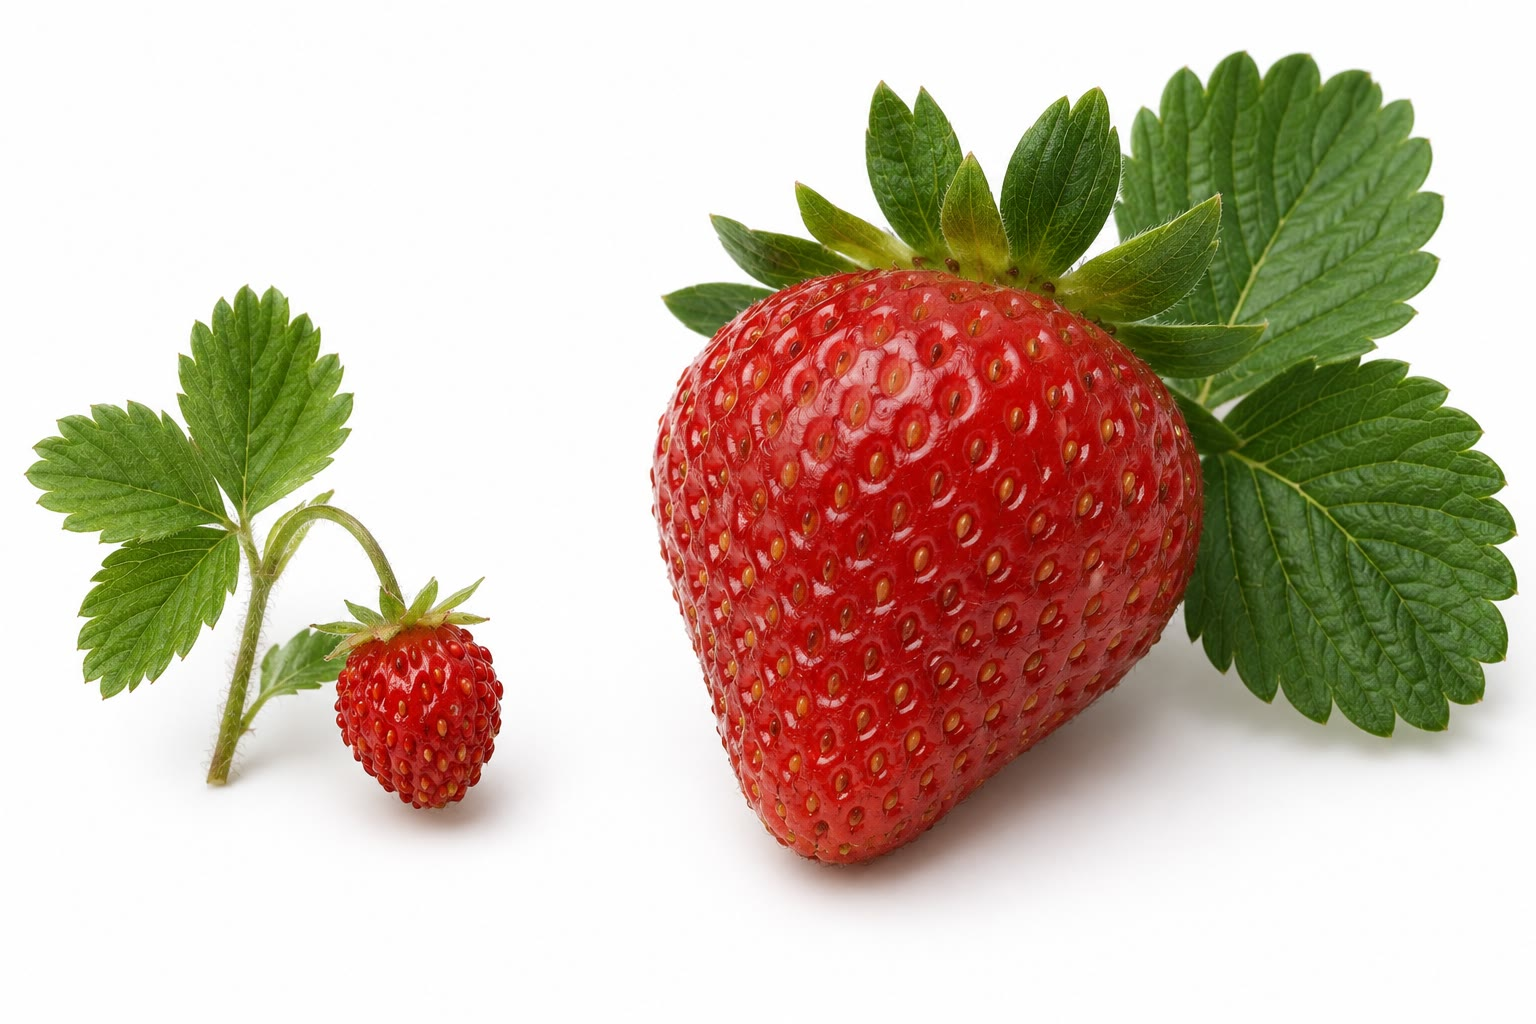
\includegraphics[width=0.55\linewidth]{images/book4/ai/b4-03-polyploid-strawberries.jpg}

{\small A wild diploid strawberry and the cultivated octoploid: the
\omterm{def:b2:genome-diversification:polyploidy}{polyploid}, with four times the DNA in every cell, is the larger
plant with the larger fruit.}
\end{omfigure}

\section{Randomness and rate}

\begin{proposition}[Mutation is random with respect to need]\label{prop:b2:genome-diversification:random}
\index{mutation!randomness of}
The \omterm{thm:b2:genome-diversification:luria}{fluctuation test} and replica plating show that a \omterm{def:b2:genome-diversification:mutation}{mutation}
useful in a new environment arises at the same rate whether or not
the environment is present: the environment selects among
\omterm{def:b2:genome-diversification:mutation}{mutations}, it does not call them forth. \omterm{def:b2:genome-diversification:mutation}{Mutation} is not random in
every sense --- transitions outnumber transversions, CpG
dinucleotides mutate ten times faster than other sites (their
methylated cytosine deaminates to thymine, which repair does not
recognise as foreign), some regions are hotspots, and stress can
raise the overall rate --- but it is blind to consequences. The
\omterm{thm:b2:genome-diversification:rate}{mutation rate} itself is a heritable trait, and selection tunes it:
too high, and each generation inherits harmful changes; too low,
and the population cannot follow a changing world. Mutator strains
win briefly in a hospital and lose in the long run, and the rate of
$10^{-9}$ per base that most cells settle on is a compromise between
the cost of errors and the cost of proofreading.
\end{proposition}

\section{Exercises}

\begin{exercise}[$\star$]\label{exo:b2:genome-diversification:1}
Classify each change to the codon GAA (glutamate): GAG; GTA; TAA;
insertion of a C after the first base. Which is a transition, which a
transversion?
\end{exercise}

\begin{exercise}[$\star$]\label{exo:b2:genome-diversification:2}
With $u = \qty{5e-10}{}$ per base pair per replication and $G =
\qty{4.6e6}{}$, how many new \omterm{def:b2:genome-diversification:mutation}{mutations} does one \emph{E.~coli}
division produce on average? How many per generation in a culture of
$10^{9}$ cells?
\end{exercise}

\begin{exercise}[$\star$]\label{exo:b2:genome-diversification:3}
Name the three routes of \omterm{def:b2:genome-diversification:hgt}{horizontal gene transfer} and say, for each,
what it requires (contact, a virus, free DNA) and what it typically
transfers.
\end{exercise}

\begin{exercise}[$\star$]\label{exo:b2:genome-diversification:4}
Distinguish autopolyploidy from allopolyploidy, with an example of
each, and explain why a diploid hybrid of two species is usually
sterile.
\end{exercise}

\begin{exercise}[$\star\star$]\label{exo:b2:genome-diversification:5}
A human germ line accumulates $u = \qty{1.2e-8}{}$ \omterm{def:b2:genome-diversification:mutation}{mutations} per
base pair per generation over a haploid genome of \qty{3.2e9}{} base
pairs. How many new \omterm{def:b2:genome-diversification:mutation}{mutations} does a child carry? If \qty{1.5}{\%}
of the genome codes for protein and \qty{70}{\%} of coding
substitutions change an amino acid, how many new amino-acid changes
does the child carry?
\end{exercise}

\begin{exercise}[$\star\star$]\label{exo:b2:genome-diversification:6}
A culture grows from $10^{3}$ to $10^{9}$ cells; a given \omterm{def:b2:genome-diversification:mutation}{mutation}
occurs at $m = \qty{2e-8}{}$ per division. Compute the expected
number of \omterm{def:b2:genome-diversification:mutation}{mutation} events and of mutant cells. Why is the fraction
of cultures with no mutant useless here for measuring $m$, and what
culture size would make it useful?
\end{exercise}

\begin{exercise}[$\star\star$]\label{exo:b2:genome-diversification:7}
Cytosine deaminates to uracil; 5-methylcytosine deaminates to
thymine. Explain why the first is efficiently repaired and the
second is not, and deduce why CpG sites (where cytosine is
methylated) are \omterm{def:b2:genome-diversification:mutation}{mutation} hotspots and are rarer in the genome than
chance would predict.
\end{exercise}

\begin{exercise}[$\star\star$]\label{exo:b2:genome-diversification:8}
In an interrupted-mating experiment, four genes enter the recipient
at 8, 17, 25 and \qty{40}{min}; the whole chromosome (\qty{4.6}{Mb})
would take \qty{100}{min}. Convert the times to positions in
kilobases and compute the distances between consecutive genes.
\end{exercise}

\begin{exercise}[$\star\star$]\label{exo:b2:genome-diversification:9}
Draw the pairing and crossing-over that turns two chromosomes with
two tandem $\alpha$-globin genes each into one with three and one
with one. A person inherits a one-gene chromosome from each parent:
how many $\alpha$ genes do they have, and what is expected of their
haemoglobin?
\end{exercise}

\begin{exercise}[$\star\star\star$]\label{exo:b2:genome-diversification:10}
Bread wheat is AABBDD with $2n = 42$. Give the chromosome number of
its gametes, of the sterile hybrids at each step of its origin, and
of a cross between bread wheat and emmer (AABB). Explain in terms of
meiotic pairing why each doubling restored fertility and why the
hexaploid cannot cross back with its parents.
\end{exercise}

\begin{exercise}[$\star\star\star$]\label{exo:b2:genome-diversification:11}
In a gut population of $N = 10^{9}$ bacteria, a resistance \omterm{def:b2:unicellular-diversity:prokaryote}{plasmid}
spreads by conjugation at a rate proportional to encounters between
carriers $R$ and non-carriers $N - R$: $\mathrm{d}R/\mathrm{d}t =
\gamma R (N - R)$ with $\gamma N = \qty{0.5}{h^{-1}}$. Solve, starting
from one carrier, and compute the time for half the population to
carry the \omterm{def:b2:unicellular-diversity:prokaryote}{plasmid}. What happens if the antibiotic is then withdrawn
and the \omterm{def:b2:unicellular-diversity:prokaryote}{plasmid} costs its host \qty{5}{\%} in growth rate?
\end{exercise}

\begin{exercise}[$\star\star\star$]\label{exo:b2:genome-diversification:12}
``\omterm{def:b2:genome-diversification:mutation}{Mutation} is random; evolution is not.'' Discuss, using the
\omterm{thm:b2:genome-diversification:luria}{fluctuation test}, replica plating, and the fact that the \omterm{thm:b2:genome-diversification:rate}{mutation
rate} is itself under selection.
\end{exercise}

\section{Problem: A Fluctuation Test}

\begin{problem}[{Weekend problem --- a fluctuation test is run and
analysed, the mutation rate of a strain extracted from it and scaled
to its genome and its population, the spread of a resistance plasmid
modelled, and the cost of a mutator weighed, ending on the strain's
mutation rate per base and the plasmid's time to take over}]
\label{pb:b2:genome-diversification:1}
Twenty cultures of \emph{E.~coli} are each started from \num{100}
cells in \qty{0.2}{mL} and grown to $N = \qty{2e8}{}$ cells; each is
then spread on a plate with a bacteriophage, and the resistant
colonies are counted: 0, 0, 0, 1, 0, 0, 3, 0, 0, 1, 0, 0, 0, 0, 107,
0, 2, 0, 0, 5. In parallel, twenty samples of \qty{0.2}{mL} are taken
from one large culture at the same density and plated likewise:
14, 15, 13, 21, 15, 14, 26, 16, 20, 13, 17, 12, 18, 14, 16, 19, 15,
13, 17, 16. Genome: \qty{4.6e6}{} base pairs, \qty{88}{\%} coding.
Resistance to the phage can arise by any one of \num{20} distinct
single-base changes in one receptor gene.

\medskip
\noindent\textbf{Part I --- The test.}
\begin{enumerate}
  \item Compute the mean and the variance of the twenty independent
        cultures.
  \item Compute the mean and the variance of the twenty samples.
  \item For a Poisson distribution the variance equals the mean.
        Which set is Poisson, and what does each set's distribution
        say about \emph{when} the \omterm{def:b2:genome-diversification:mutation}{mutations} occurred?
  \item Explain the count of 107.
  \item How many of the independent cultures contain no mutant? Use
        $p_0 = e^{-m(N - N_0)}$ to estimate $m$, the \omterm{thm:b2:genome-diversification:rate}{mutation rate} to
        resistance per cell division.
  \item Compute the expected number of mutant cells per culture from
        $mN\ln(N/N_0)$ and compare with the observed mean.
  \item Why would the samples from the single culture have been
        useless for estimating $m$ by the $p_0$ method?
\end{enumerate}

\medskip
\noindent\textbf{Part II --- Scaling to the genome.}
\begin{enumerate}[resume]
  \item Deduce the \omterm{thm:b2:genome-diversification:rate}{mutation rate} $u$ per base pair per replication
        from $m$ and the number of resistance-conferring changes.
  \item Compute the mean number of new \omterm{def:b2:genome-diversification:mutation}{mutations} per genome per
        replication, $U$.
  \item A one-litre culture at $10^{9}$ cells per millilitre doubles
        once. How many new \omterm{def:b2:genome-diversification:mutation}{mutations} arise in the population?
  \item How many distinct single-base changes are possible in this
        genome? On average, how many times does each arise in that
        one doubling?
  \item Explain why, in such a population, resistance to any single
        antibiotic that one \omterm{def:b2:genome-diversification:mutation}{mutation} can defeat is essentially
        guaranteed to be present.
  \item Explain why combining two antibiotics that need two
        independent \omterm{def:b2:genome-diversification:mutation}{mutations} changes this, with a number.
\end{enumerate}

\medskip
\noindent\textbf{Part III --- A \omterm{def:b2:unicellular-diversity:prokaryote}{plasmid} spreads.}
In a gut holding $N = 10^{9}$ cells, one cell acquires a conjugative
resistance \omterm{def:b2:unicellular-diversity:prokaryote}{plasmid}. Carriers $R$ transmit it on contact:
$\mathrm{d}R/\mathrm{d}t = \gamma R(N - R)$, with $\gamma N =
\qty{0.5}{h^{-1}}$.
\begin{enumerate}[resume]
  \item Show that $R(t) = N/\bigl(1 + (N - 1)e^{-\gamma N t}\bigr)$
        solves the equation with $R(0) = 1$.
  \item Compute the time at which half the cells carry the \omterm{def:b2:unicellular-diversity:prokaryote}{plasmid}.
  \item Compute the time at which \qty{99}{\%} do.
  \item How many conjugation events per hour take place at the moment
        when half the cells are carriers?
  \item Compare with the time for a resistant \emph{mutant} to reach
        half the population by growing \qty{10}{\%} faster than the
        rest under the antibiotic (\omterm{def:b2:unicellular-diversity:division}{generation time} \qty{1}{h} for the
        sensitive cells): starting from one cell, how long does it
        take?
  \item Conclude on why resistance spreads mainly by transfer rather
        than by descent.
\end{enumerate}

\medskip
\noindent\textbf{Part IV --- A mutator.}
A strain lacking mismatch repair mutates \num{100} times faster.
Suppose \qty{30}{\%} of \omterm{def:b2:genome-diversification:mutation}{mutations} in coding sequence are harmful.
\begin{enumerate}[resume]
  \item Compute its $U$ and the mean number of harmful \omterm{def:b2:genome-diversification:mutation}{mutations} per
        cell per generation.
  \item After \num{200} generations, what fraction of a lineage's
        descendants carry no harmful \omterm{def:b2:genome-diversification:mutation}{mutation} at all (Poisson)?
  \item Compute the same for the wild type.
  \item In the \omterm{thm:b2:genome-diversification:luria}{fluctuation test} above, what mean count would the
        mutator have given, and what fraction of cultures with no
        mutant?
  \item Explain in two sentences why mutators are found among
        hospital isolates and are rare in nature.
  \item State the result: $m$, $u$, $U$ for the strain, and the times
        for the \omterm{def:b2:unicellular-diversity:prokaryote}{plasmid} to reach half and \qty{99}{\%} of the gut.
\end{enumerate}
\end{problem}
